% Options for packages loaded elsewhere
\PassOptionsToPackage{unicode}{hyperref}
\PassOptionsToPackage{hyphens}{url}
%
\documentclass[
]{book}
\usepackage{lmodern}
\usepackage{amssymb,amsmath}
\usepackage{ifxetex,ifluatex}
\ifnum 0\ifxetex 1\fi\ifluatex 1\fi=0 % if pdftex
  \usepackage[T1]{fontenc}
  \usepackage[utf8]{inputenc}
  \usepackage{textcomp} % provide euro and other symbols
\else % if luatex or xetex
  \usepackage{unicode-math}
  \defaultfontfeatures{Scale=MatchLowercase}
  \defaultfontfeatures[\rmfamily]{Ligatures=TeX,Scale=1}
\fi
% Use upquote if available, for straight quotes in verbatim environments
\IfFileExists{upquote.sty}{\usepackage{upquote}}{}
\IfFileExists{microtype.sty}{% use microtype if available
  \usepackage[]{microtype}
  \UseMicrotypeSet[protrusion]{basicmath} % disable protrusion for tt fonts
}{}
\makeatletter
\@ifundefined{KOMAClassName}{% if non-KOMA class
  \IfFileExists{parskip.sty}{%
    \usepackage{parskip}
  }{% else
    \setlength{\parindent}{0pt}
    \setlength{\parskip}{6pt plus 2pt minus 1pt}}
}{% if KOMA class
  \KOMAoptions{parskip=half}}
\makeatother
\usepackage{xcolor}
\IfFileExists{xurl.sty}{\usepackage{xurl}}{} % add URL line breaks if available
\IfFileExists{bookmark.sty}{\usepackage{bookmark}}{\usepackage{hyperref}}
\hypersetup{
  pdftitle={金融数学},
  pdfauthor={Financial Mathematics},
  hidelinks,
  pdfcreator={LaTeX via pandoc}}
\urlstyle{same} % disable monospaced font for URLs
\usepackage{longtable,booktabs}
% Correct order of tables after \paragraph or \subparagraph
\usepackage{etoolbox}
\makeatletter
\patchcmd\longtable{\par}{\if@noskipsec\mbox{}\fi\par}{}{}
\makeatother
% Allow footnotes in longtable head/foot
\IfFileExists{footnotehyper.sty}{\usepackage{footnotehyper}}{\usepackage{footnote}}
\makesavenoteenv{longtable}
\usepackage{graphicx,grffile}
\makeatletter
\def\maxwidth{\ifdim\Gin@nat@width>\linewidth\linewidth\else\Gin@nat@width\fi}
\def\maxheight{\ifdim\Gin@nat@height>\textheight\textheight\else\Gin@nat@height\fi}
\makeatother
% Scale images if necessary, so that they will not overflow the page
% margins by default, and it is still possible to overwrite the defaults
% using explicit options in \includegraphics[width, height, ...]{}
\setkeys{Gin}{width=\maxwidth,height=\maxheight,keepaspectratio}
% Set default figure placement to htbp
\makeatletter
\def\fps@figure{htbp}
\makeatother
\setlength{\emergencystretch}{3em} % prevent overfull lines
\providecommand{\tightlist}{%
  \setlength{\itemsep}{0pt}\setlength{\parskip}{0pt}}
\setcounter{secnumdepth}{5}
\usepackage{booktabs}
\usepackage{ctex}
\usepackage{amsthm}
\makeatletter
\def\thm@space@setup{%
  \thm@preskip=8pt plus 2pt minus 4pt
  \thm@postskip=\thm@preskip
}
\makeatother
\usepackage{flafter}
\usepackage[]{natbib}
\bibliographystyle{apalike}

\title{金融数学}
\author{Financial Mathematics}
\date{2020-10-09 14:19:50}

\begin{document}
\maketitle

{
\setcounter{tocdepth}{1}
\tableofcontents
}
\hypertarget{ux6b22ux8fce}{%
\chapter*{👨‍🏫 欢迎}\label{ux6b22ux8fce}}
\addcontentsline{toc}{chapter}{👨‍🏫 欢迎}

在这里,我们同步课堂,总结每章的\textbf{重点、难点},并发布\textbf{课后作业}。课后作业需在下次上课交到讲台上。

我们这里主要以英文表述,有以下两个原因

\begin{enumerate}
\def\labelenumi{\arabic{enumi}.}
\item
  方便大家准备SOA/CAS的 \href{https://www.soa.org/education/exam-req/edu-exam-fm-detail/}{Exam FM: Financial Mathematics} 考试;
\item
  方便大家阅读相关英文文献。
\end{enumerate}

此网站由授课老师高光远、助教程轶鹏、助教胡夏新管理,欢迎大家反馈意见到助教、微信群、或邮箱 \href{mailto:guangyuan.gao@ruc.edu.cn}{\nolinkurl{guangyuan.gao@ruc.edu.cn}}。

\hypertarget{ux7b54ux7591}{%
\section*{🤔 答疑}\label{ux7b54ux7591}}
\addcontentsline{toc}{section}{🤔 答疑}

\textbf{我定期把同学们的普遍疑问在这里解答,欢迎提问!}

\textbf{👉 期末中文考题} (2020/09/26)

\begin{center}
\includegraphics[width=0.3\linewidth]{./plots/english} \end{center}

\textbf{👉 证明\(\frac{1}{a_{\overline{n}\mid}}=\frac{1}{s_{\overline{n}\mid}}+i\)} (2020/09/24)

假设有A, B, C三种年金:

\begin{itemize}
\item
  A:\(n\)年期期末付等额年金,一共\(n\)个\(\frac{1}{a_{\overline{n}\mid}}\),分别在\(t=1,\ldots,n\)。A的现值为\[\frac{1}{a_{\overline{n}\mid}} a_{\overline{n}\mid}=1\]
\item
  B:\(n\)年期期末付年金,一共\(n-1\)个\(i\)和一个\(1+i\), 分别在\(t=1,\ldots,n\)。 B的现值为\[ia_{\overline{n}\mid}+v^n=1.\]
\item
  C:C为B的``平滑''化年金,即把在时间\(t=n\)的1转化为\(n\)个在\(t=1,\ldots,n\)的等额年金(其在\(t=n\)的累计值应为1),所以分摊到每个时刻的金额为\(\frac{1}{s_{\overline{n}\mid}}\)。 ``平滑''后的年金为\(n\)年期期末付等额年金,一共\(n\)个\(\frac{1}{s_{\overline{n}\mid}}+i\)。 C和B的现值相同都为1。
\end{itemize}

可见,A和C同为\(n\)年期期末付等额年金,其现值都为1。所以,它们每期的金额也应该相同:
\[\frac{1}{a_{\overline{n}\mid}}=\frac{1}{s_{\overline{n}\mid}}+i.\]

\textbf{👉 \(i\) 和 \(d\) 的关系} (2020/09/16)

很多同学问课件上的这道题目。

问题:已知年实际利率为5\%。回答下述问题:

(1)100万元贷款在年末的利息是多少?\(100\times5%
\)

(2)如果在贷款起始日收取利息,应该收取多少利息?\(100\times i/(1+i)=100\times d\)

(3)年实际贴现率是多少?\(d=i/(1+i)\)

\(i\) 和 \(d\) 的区别可以理解为 \(i\) 是在\textbf{期末}付,\(d\) 是在\textbf{期初}付。\(d=i\times v\),即期末 \(i\) 的\textbf{现值}是 \(d\)。

所以(1)是期末收的利息,(2)是期初收的利息。期初收的利息要比期末收的少,因为银行收到的这部分利息在这一年中还能产生利息,期初收的 \(d\) 到期末是 \(i\)。

贴现率 \(d\) 的另一种理解就是利息 \(i\) 的现值。

\textbf{👉 计算器} (2020/09/10)

在课堂测验和期末考试,没有对计算器的严格要求,但至少需要科学计算器。大家不需要购买昂贵的可编程计算器,在这门课中,体现不出可编程计算器的优势。

建议的计算器是SOA/CAS要求的\href{https://www.soa.org/education/exam-req/exam-day-info/edu-id-calculators/}{计算器}。

\textbf{👉 最终成绩} (2020/09/10)

\begin{enumerate}
\def\labelenumi{\arabic{enumi}.}
\item
  平时成绩占40\%,期末成绩占60\%。
\item
  平时成绩主要根据课堂点名、课外作业的完成态度、随堂测试的准确度评定。
\end{enumerate}

\hypertarget{interest-rate}{%
\chapter{Interest rate}\label{interest-rate}}

\hypertarget{key-concepts}{%
\section{Key concepts}\label{key-concepts}}

\hypertarget{functions}{%
\subsection*{Functions}\label{functions}}
\addcontentsline{toc}{subsection}{Functions}

\begin{itemize}
\item
  Accumulation function \[a(t)\]
\item
  Discount function \[a^{-1}(t)\]
\end{itemize}

\hypertarget{interest-rate-1}{%
\subsection*{Interest rate}\label{interest-rate-1}}
\addcontentsline{toc}{subsection}{Interest rate}

\begin{itemize}
\item
  Effective rate of interest/discount \[i,d\]
\item
  Simple interest \[a(t)=1+it\]
\item
  Compound interest \[a(t)=(1+i)^t\]
\item
  Discount factor \[v=(1+i)^{-1}\]
\item
  Accumulation factor of \(t\) years \[(1+i)^t\]
\item
  Discount factor of \(t\) years \[(1+i)^{-t}\]
\item
  Nominal rate of interest/discount \[i^{(m)},d^{(m)}\]
\item
  Force of interest \[\delta\]
\end{itemize}

\hypertarget{values}{%
\subsection*{Values}\label{values}}
\addcontentsline{toc}{subsection}{Values}

\begin{itemize}
\item
  Accumulated value (future value)
\item
  Present value
\end{itemize}

\hypertarget{key-equations}{%
\section{Key equations}\label{key-equations}}

\hypertarget{accumulation-and-discount}{%
\subsection*{Accumulation and discount}\label{accumulation-and-discount}}
\addcontentsline{toc}{subsection}{Accumulation and discount}

\[a(t)=(1+i)^t=(1-d)^{-t}\]

\[a^{-1}(t)=(1+i)^{-t}=(1-d)^t=v^t\]

\hypertarget{effective-interest-rate-and-discount-rate}{%
\subsection*{Effective interest rate and discount rate}\label{effective-interest-rate-and-discount-rate}}
\addcontentsline{toc}{subsection}{Effective interest rate and discount rate}

\[i=\frac{d}{1-d}\]

\[d=\frac{i}{1+i}\]

\[d=iv\]

\[v=1-d\]

\[i-d=id\]

\hypertarget{nominal-interest-rate-and-effective-interest-rate}{%
\subsection*{Nominal interest rate and effective interest rate}\label{nominal-interest-rate-and-effective-interest-rate}}
\addcontentsline{toc}{subsection}{Nominal interest rate and effective interest rate}

\[1+i=\left(1+\frac{i^{(m)}}{m}\right)^m\]
\[1-d=\left(1-\frac{d^{(m)}}{m}\right)^m\]
\[d^{(m)}=i^{(m)}\times\left(1+\frac{i^{(m)}}{m}\right)^{-1}\]

\hypertarget{force-of-interest}{%
\subsection*{Force of interest}\label{force-of-interest}}
\addcontentsline{toc}{subsection}{Force of interest}

\[\delta(t)=\frac{a'(t)}{a(t)}\]

\[a(t)=e^{\int_0^t\delta(s)ds}\]

\[\delta=\ln(1+i)\]
\[\delta=\lim_{m\rightarrow\infty} i^{(m)}=\lim_{m\rightarrow\infty} d^{(m)}=\ln(1+i)\]

\[d\le d^{(2)}\le d^{(3)}\le\cdots\le \delta\le\cdots\le i^{(3)}\le i^{(2)}\le i\]

\hypertarget{level-annuity}{%
\chapter{Level annuity}\label{level-annuity}}

\hypertarget{key-concepts}{%
\section{Key concepts}\label{key-concepts}}

\hypertarget{annuity-immediate}{%
\subsection*{Annuity immediate}\label{annuity-immediate}}
\addcontentsline{toc}{subsection}{Annuity immediate}

\[a_{\overline{n}\mid}=\frac{1-v^n}{i}\]
\[s_{\overline{n}\mid}=(1+i)^na_{\overline{n}\mid}=\frac{(1+i)^n-1}{i}\]

\hypertarget{annuity-due}{%
\subsection*{Annuity due}\label{annuity-due}}
\addcontentsline{toc}{subsection}{Annuity due}

\[\ddot{a}_{\overline{n}\mid}=\frac{1-v^n}{d}=(1+i)a_{\overline{n}\mid}=1+a_{\overline{n-1}\mid}\]

\[\ddot{s}_{\overline{n}\mid}=(1+i)^n\ddot{a}_{\overline{n}\mid}\]

\hypertarget{deffered-annuity}{%
\subsection*{Deffered annuity}\label{deffered-annuity}}
\addcontentsline{toc}{subsection}{Deffered annuity}

\[_{m|}a_{\overline{n}\mid}=v^ma_{\overline{n}\mid}=a_{\overline{m+n}\mid}-a_{\overline{n}\mid}\]

\hypertarget{perpetuity}{%
\subsection*{Perpetuity}\label{perpetuity}}
\addcontentsline{toc}{subsection}{Perpetuity}

\[a_{\overline{\infty}\mid}=\frac{1}{i}\]
\[\ddot{a}_{\overline{\infty}\mid}=\frac{1}{d}\]

\hypertarget{m-thly-payable-annuity}{%
\subsection*{\texorpdfstring{\(m\)-thly payable annuity}{m-thly payable annuity}}\label{m-thly-payable-annuity}}
\addcontentsline{toc}{subsection}{\(m\)-thly payable annuity}

\[a^{(m)}_{\overline{n}\mid}=\frac{1-v^n}{i^{(m)}}=\frac{i}{i^{(m)}}a_{\overline{n}\mid}\]
\[\ddot{a}^{(m)}_{\overline{n}\mid}=\frac{1-v^n}{d^{(m)}}=\frac{d}{d^{(m)}}a_{\overline{n}\mid}\]
\[a^{(m)}_{\overline{\infty}\mid}=\frac{1}{i^{(m)}}\]
\[\ddot{a}^{(m)}_{\overline{\infty}\mid}=\frac{1}{d^{(m)}}\]
\[\ddot{a}^{(m)}_{\overline{\infty}\mid}=(1+i)^{1/m}a^{(m)}_{\overline{\infty}\mid}\]

\hypertarget{continuous-payable-annuity}{%
\subsection*{Continuous payable annuity}\label{continuous-payable-annuity}}
\addcontentsline{toc}{subsection}{Continuous payable annuity}

\[\bar{a}_{\overline{n}\mid}=\frac{i}{\delta}{a}_{\overline{n}\mid}=\frac{d}{\delta}\ddot{a}_{\overline{n}\mid}=\frac{1-v^n}{\delta}\]
\[\bar{a}_{\overline{\infty}\mid}=\frac{1}{\delta}\]

\hypertarget{key-relations}{%
\section{Key relations}\label{key-relations}}

\begin{center}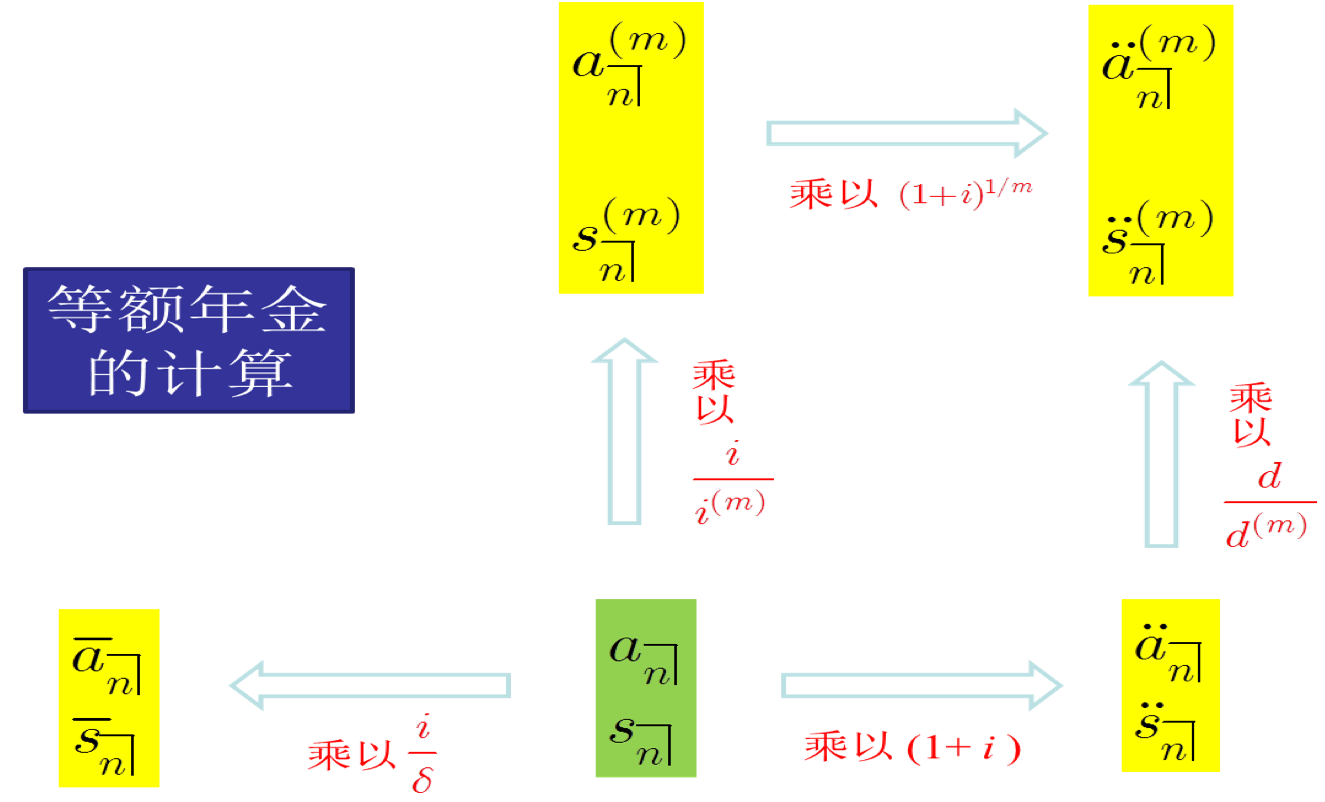
\includegraphics[width=0.5\linewidth]{./plots/annuity-1} \end{center}

\hypertarget{homework}{%
\chapter*{🖊️ Homework}\label{homework}}
\addcontentsline{toc}{chapter}{🖊️ Homework}

\hypertarget{week-5}{%
\section*{Week 5}\label{week-5}}
\addcontentsline{toc}{section}{Week 5}

\hypertarget{problem-1}{%
\subsection*{Problem 1}\label{problem-1}}
\addcontentsline{toc}{subsection}{Problem 1}

\emph{SOA 11/01 \#16}

Olga buys a \(5\)-year increasing annuity for \(X\). Olga will receive \(2\) at the end of the first month, \(4\) at the end of the second month, and for each month thereafter the payment increases by \(2\). The nominal interest rate is \(9\%\) convertible quarterly. Calculate \(X\).

\hypertarget{problem-2}{%
\subsection*{Problem 2}\label{problem-2}}
\addcontentsline{toc}{subsection}{Problem 2}

\emph{SOA 5/95 \#7}

The first payment of a perpetuity-immediate is \(60\). Subsequent payments decrease by \(1\) per year until they reach a level of \(k\). Payments remain constant at \(k\) thereafter. The present value of the perpetuity is equal to the present of a perpetuity-immediate paying \(44\) each year. The annual effective interest rate is \(5\%\). Calculate \(k\).

\hypertarget{problem-3}{%
\subsection*{Problem 3}\label{problem-3}}
\addcontentsline{toc}{subsection}{Problem 3}

\emph{SOA 11/01 \#5}

Mike buys a perpetuity-immediate with varying annual payments. During the first \(5\) years, the payment is constant and equal to \(10\). Beginning in year \(6\), the payments start to increase. For year \(6\) and all future years, the current year's payment is \(K\%\) larger than the previous year's payment. At an annual effective interest rate of \(9.2\%\), the perpetuity has a present value of \(167.50\). Calculate \(K\), given \(K < 9.2\).

\hypertarget{week-3}{%
\section*{Week 3}\label{week-3}}
\addcontentsline{toc}{section}{Week 3}

\hypertarget{problem-1-1}{%
\subsection*{Problem 1}\label{problem-1-1}}
\addcontentsline{toc}{subsection}{Problem 1}

\emph{SAMPLE/00 \#27}

Susan and Jeff each make deposits of \(100\) at the end of each year for \(40\) years.

Starting at the end of the \(41st\) year, Susan makes annual withdrawals of \(X\) for \(15\) years and Jeff makes annual withdrawals of \(Y\) for \(15\) years. Both funds have a balance of \(0\) after the last withdrawal.

Susan's fund earns an annual effective interest rate of \(8\%\). Jeff's fund earns an annual effective interest rate at \(10\%\).

Calculate \(Y-X\).

\hypertarget{problem-2-1}{%
\subsection*{Problem 2}\label{problem-2-1}}
\addcontentsline{toc}{subsection}{Problem 2}

\emph{SOA 11/01 \#27}

A man turns \(40\) today and wishes to provide supplemental retirement income of \(3000\) at the beginning of each month starting on his 65th birthday. Starting today, he makes monthly contributions of \(X\) to a fund for \(25\) years.

The fund earns a nominal rate of \(8\%\) compounded monthly. Each \(1000\) will provide for \(9.65\) income at the beginning of month starting on his 65th birthday until the end of his life.

Calculate \(X\).

\hypertarget{problem-3-1}{%
\subsection*{Problem 3}\label{problem-3-1}}
\addcontentsline{toc}{subsection}{Problem 3}

\emph{SOA 11/93 \#4}

At time \(t=0\), Paul deposits \(P\) into a fund crediting interest at an effective annual interest rate of \(8\%\). At the end of each year in years \(6\) through \(20\), Paul withdraws an amount sufficient to purchase an annuity-due of \(100\) per month for \(10\) years at a nominal interest rate of \(12\%\) compounded monthly. Immediately after the withdrawal at the end of year \(20\), the fund value is zero.

Calculate \(P\).

\hypertarget{week-2}{%
\section*{Week 2}\label{week-2}}
\addcontentsline{toc}{section}{Week 2}

\hypertarget{problem-1-2}{%
\subsection*{Problem 1}\label{problem-1-2}}
\addcontentsline{toc}{subsection}{Problem 1}

\emph{SOA 5/98 \#2}

John invests \(1000\) in a fund which earns interest during the first year at a nominal rate of \(K\) convertible quarterly. During the 2nd year the fund earns interest at a nominal discount rate of \(K\) convertible quarterly. At the end of the 2nd year,the fund has accumulated to \(1173.54\).

Calculate \(K\).

\hypertarget{problem-2-2}{%
\subsection*{Problem 2}\label{problem-2-2}}
\addcontentsline{toc}{subsection}{Problem 2}

\emph{SOA 5/89 \#4}

Two funds,\(X\) and \(Y\),start with the same amount.You are given:

\begin{enumerate}
\def\labelenumi{\arabic{enumi}.}
\item
  Fund \(X\) accumulates at a force of interest of 5\%.
\item
  Fund \(Y\) accumulates at a rate of interest \(j\), compounded semiannually.
\item
  At the end of eight years, Fund \(X\) is \(1.05\) times as large as Fund \(Y\).
\end{enumerate}

Calculate \(j\).

\hypertarget{problem-3-2}{%
\subsection*{Problem 3}\label{problem-3-2}}
\addcontentsline{toc}{subsection}{Problem 3}

\emph{SOA 11/89 \#2}

Fund \(X\) starts with \(1,000\) and accumulates with a force of interest \[\delta_{t}=\frac{1}{15-t} \text{ for } 0 \le t< 15.\]

Fund Y starts with \(1,000\) and accumulates with an interest rate of 8\% per annum compounded semiannually for the first three years and an effective interest rate of \(i\) per annum thereafter.

Fund \(X\) equals Fund \(Y\) at the end of four years.

Calculate \(i\).

\hypertarget{week-1}{%
\section*{Week 1}\label{week-1}}
\addcontentsline{toc}{section}{Week 1}

\hypertarget{problem-1-3}{%
\subsection*{Problem 1}\label{problem-1-3}}
\addcontentsline{toc}{subsection}{Problem 1}

John invests \(X\) in a fund growing in accordance with the accumulation function implied by the \emph{amount function}
\[A(t)=4t^2+8t+4.\]
Edna invests \(X\) in another fund growing in accordance with the accumulation function implied by the amount function \[A(t)=4t^2+2.\]
When does Edna's investment \emph{exceed} John's?

\hypertarget{problem-2-3}{%
\subsection*{Problem 2}\label{problem-2-3}}
\addcontentsline{toc}{subsection}{Problem 2}

What deposit made today will provide for a payment of \(\$1000\) in 1 year and \(\$2000\) in 3 years, if the effective rate of interest is \(7.5\%\)?

\hypertarget{problem-3-3}{%
\subsection*{Problem 3}\label{problem-3-3}}
\addcontentsline{toc}{subsection}{Problem 3}

Company \(X\) received the approval to start no more than two projects in the current calendar year.
Three different projects were recommended, each of which requires an investment of 800 to be made at the beginning of the year.

The cash flows for each of the three projects are shown in Table \ref{tab:week1}:

\begin{table}[!h]

\caption{\label{tab:week1}The cash flows of the three projects.}
\centering
\begin{tabular}[t]{r|r|r|r}
\hline
End of year & Project A & Project B & Project C\\
\hline
1 & 500 & 500 & 500\\
\hline
2 & 500 & 300 & 250\\
\hline
3 & -175 & -175 & -175\\
\hline
4 & 100 & 150 & 200\\
\hline
5 & 0 & 200 & 200\\
\hline
\end{tabular}
\end{table}

The company uses an annual effective interest rate of \(10\%\) to discount its cash flows.

Determine which combination of projects the company should select.

\hypertarget{solutions-to-homework}{%
\chapter*{💡 Solutions to homework}\label{solutions-to-homework}}
\addcontentsline{toc}{chapter}{💡 Solutions to homework}

\hypertarget{week-2}{%
\section*{Week 2}\label{week-2}}
\addcontentsline{toc}{section}{Week 2}

\hypertarget{problem-1}{%
\subsection*{Problem 1}\label{problem-1}}
\addcontentsline{toc}{subsection}{Problem 1}

AV in 2 years = 1173.54, so we set:
\[1173.54=1000\left(1+\frac{K}{4}\right)^{4}\left(1-\frac{K}{4}\right)^{-4}=1000\left(\frac{4+K}{4-K}\right)^{4}\]
Thus,
\[\frac{4+K}{4-K}=1.17354^{1/4}=1.0408\]
Solving for K, we get:
\[K=0.08\]

\hypertarget{problem-2}{%
\subsection*{Problem 2}\label{problem-2}}
\addcontentsline{toc}{subsection}{Problem 2}

AV in 8 years:

\textbf{Fund X}:\[e^{(0.05)(8)}=e^{0.4}\]
\textbf{Fund Y}:\[\left(1+\frac{j}{2}\right)^{(2)(8)}=\left(1+\frac{j}{2}\right)^{16}\]
At the end of eight years, Fund \(X\) is 1.05 times as large as Fund \(Y\), so we set:
\[e^{0.4}=1.05\left(1+\frac{j}{2}\right)^{16}\]
Thus,
\[j=2\left[\left(\frac{e^{0.4}}{1.05}\right)^{\frac{1}{16}}-1\right]=0.044\]

\hypertarget{problem-3}{%
\subsection*{Problem 3}\label{problem-3}}
\addcontentsline{toc}{subsection}{Problem 3}

Fund \(X\) equals Fund \(Y\) at the end of four years, so we set:
\[1000(1.04)^{6}(1+i)=1000e^{\int_{0}^{4} \frac{1}{(15-t)} dt}\]
Then,
\[1000e^{\int_{0}^{4} \frac{1}{(15-t)} dt}=1000e^{-\ln(15-t)|_{0}^{4}}=1000\left(\frac{15}{11}\right)\]

Thus,
\[(1+i)=\frac{15}{(11)(1.04)^6}=1.0777\]
\[i=0.0777\]

\hypertarget{week-1}{%
\section*{Week 1}\label{week-1}}
\addcontentsline{toc}{section}{Week 1}

\hypertarget{problem-1-1}{%
\subsection*{Problem 1}\label{problem-1-1}}
\addcontentsline{toc}{subsection}{Problem 1}

To compare the two funds, we assume that equal investments of \(X\) are made at time 0.

John's \textbf{accumulation function} is \[t^2+2t+1\]

Edna's \textbf{accumulation function} is \[2t^{2}+1\]

To determine when Edna's investment exceeds John's, we set:

\[ X(2t^{2}+1)>X(t^{2}+2t+1)\]

which reduces to:

\[t^{2}-2t>0\] or \[t(t-2)>0\]

Thus, Edna's fund exceeds John's after 2 years.

\hypertarget{problem-2-1}{%
\subsection*{Problem 2}\label{problem-2-1}}
\addcontentsline{toc}{subsection}{Problem 2}

\[PV=1000v+2000v^{3}=2540.15 \]

since \[v=1.075^{-1}\]

\hypertarget{problem-3-1}{%
\subsection*{Problem 3}\label{problem-3-1}}
\addcontentsline{toc}{subsection}{Problem 3}

Discounting at \(10\%\), the net present values are \(4.59\),\(-2.36\) and \(-9.54\) for Projects A,B,and C respectively.

Take Project A as an example:

\[NPV=-800+500v+500v^{2}-175v^{3}+100v^{4}=4.59\]

since \[v=1.10^{-1}\]

Hence, only Project A should be funded.

  \bibliography{\_reference.bib}

\end{document}
